\documentclass[conference]{IEEEtran}
\usepackage{graphicx}
\usepackage{booktabs}
\usepackage{amsmath}
\usepackage{amssymb}
\usepackage{hyperref}
\usepackage{xcolor}
\usepackage{colortbl}
\usepackage{multirow}
\usepackage{array}
\usepackage{caption}

\hypersetup{
    colorlinks=true,
    linkcolor=blue,
    citecolor=blue,
    urlcolor=blue
}

\begin{document}

\title{Quantifying Spurious Grounding Robustness in Retrieval-Augmented Language Models: A Reproduction and Inference-Time Filtering Investigation}

\author{
    \IEEEauthorblockN{Siddhartha Shukla, Piyush Kaushal, Sugat Athawale, Ayush Dev}
    \IEEEauthorblockA{Department of Computer Science \& Artificial Intelligence\\
    Rishihood University (Newton School of Technology)\\
    Sonipat, Haryana, India\\
    Repository: \url{https://github.com/SiddharthaShukla8/NLP_Project}}
}

\maketitle

\begin{abstract}
Retrieval-Augmented Generation (RAG) integrates non-parametric retrieval corpora with parametric neural language models to anchor responses in external factual context and mitigate hallucination. However, recent benchmarks such as the SURE framework reveal that Retrieval-Augmented Language Models (RALMs) are acutely vulnerable to implicit, non-causal \textit{spurious features} embedded within retrieved grounding passages. In this paper, we investigate the empirical mechanics of this vulnerability and rigorously evaluate a zero-shot, inference-time preprocessing intervention designed to neutralize query-correlated distractors without requiring parameter fine-tuning. Using an extractive reader baseline (\texttt{deepset/roberta-base-squad2}) on the SQuAD v2.0 benchmark, we first replicate the core vulnerability phenomenon, measuring an Exact Match (EM) degradation from $68.00\%$ under clean gold context down to $54.00\%$ under query-correlated distractor injection (a $14.00\%$ robustness drop). We then formulate and pre-register a formal hypothesis: that filtering candidate context sentences exhibiting high directional keyword overlap ($\tau = 0.3$) prior to inference would eliminate spurious attention hijacking and recover $8.00\%\text{--}12.00\%$ EM. Controlled empirical evaluation conclusively refutes this hypothesis: token-overlap filtering causes reader performance to collapse catastrophically to $16.00\%$ EM (a net degradation of $-38.00\%$ relative to the unfiltered noisy condition). A systematic 5-point parameter ablation sweep ($\tau \in [0.1, 0.5]$) and a $2\times2$ error transition audit reveal that naive lexical overlap is an intrinsically confounded heuristic, inflicting a devastating $44.0\%$ collateral deletion rate on authentic gold evidence sentences. We conclude that surface lexical heuristics cannot separate spurious noise from evidentiary facts, demonstrating that robust inference-time RAG defense requires deep semantic entailment modeling rather than keyword pruning.
\end{abstract}

\begin{IEEEkeywords}
Retrieval-Augmented Generation, Spurious Features, RAG Robustness, Question Answering, Natural Language Processing, Failure Analysis.
\end{IEEEkeywords}

\section{Introduction}
Retrieval-Augmented Generation (RAG) has rapidly established itself as the standard architectural paradigm for grounding Large Language Models (LLMs) in up-to-date, verifiable factual knowledge. By dynamically fetching non-parametric text passages from an external corpus and prepending them to the user's prompt, RAG pipelines mitigate parametric hallucinations, expand temporal coverage, and facilitate transparent attribution in high-stakes domain deployments. Despite these clear advantages, contemporary RAG systems remain remarkably brittle when operating in noisy, unstructured real-world environments where retrieval engines inevitably return imperfect, partially relevant, or adversarial documentation.

While earlier literature predominantly characterized retrieval noise as \textit{semantic irrelevance}---consisting of off-topic documents or blatant factual contradictions---recent findings formalized by Yang et al.~\cite{yang2026spurious} demonstrate that models are equally, if not more, susceptible to \textit{spurious features}. Spurious features represent non-causal, surface-level textual artifacts such as authoritative styling, metadata markers, or dense keyword overlap that correlate superficially with the user's query without providing genuine evidentiary support for the answer. When such carrier sentences are injected into grounding context (as illustrated in Fig.~\ref{fig:rag_pipeline}), the cross-attention mechanisms of neural reader models disproportionately focus on the distractor tokens, drawing the model away from the true factual answer span.

\begin{figure}[htbp]
\centering
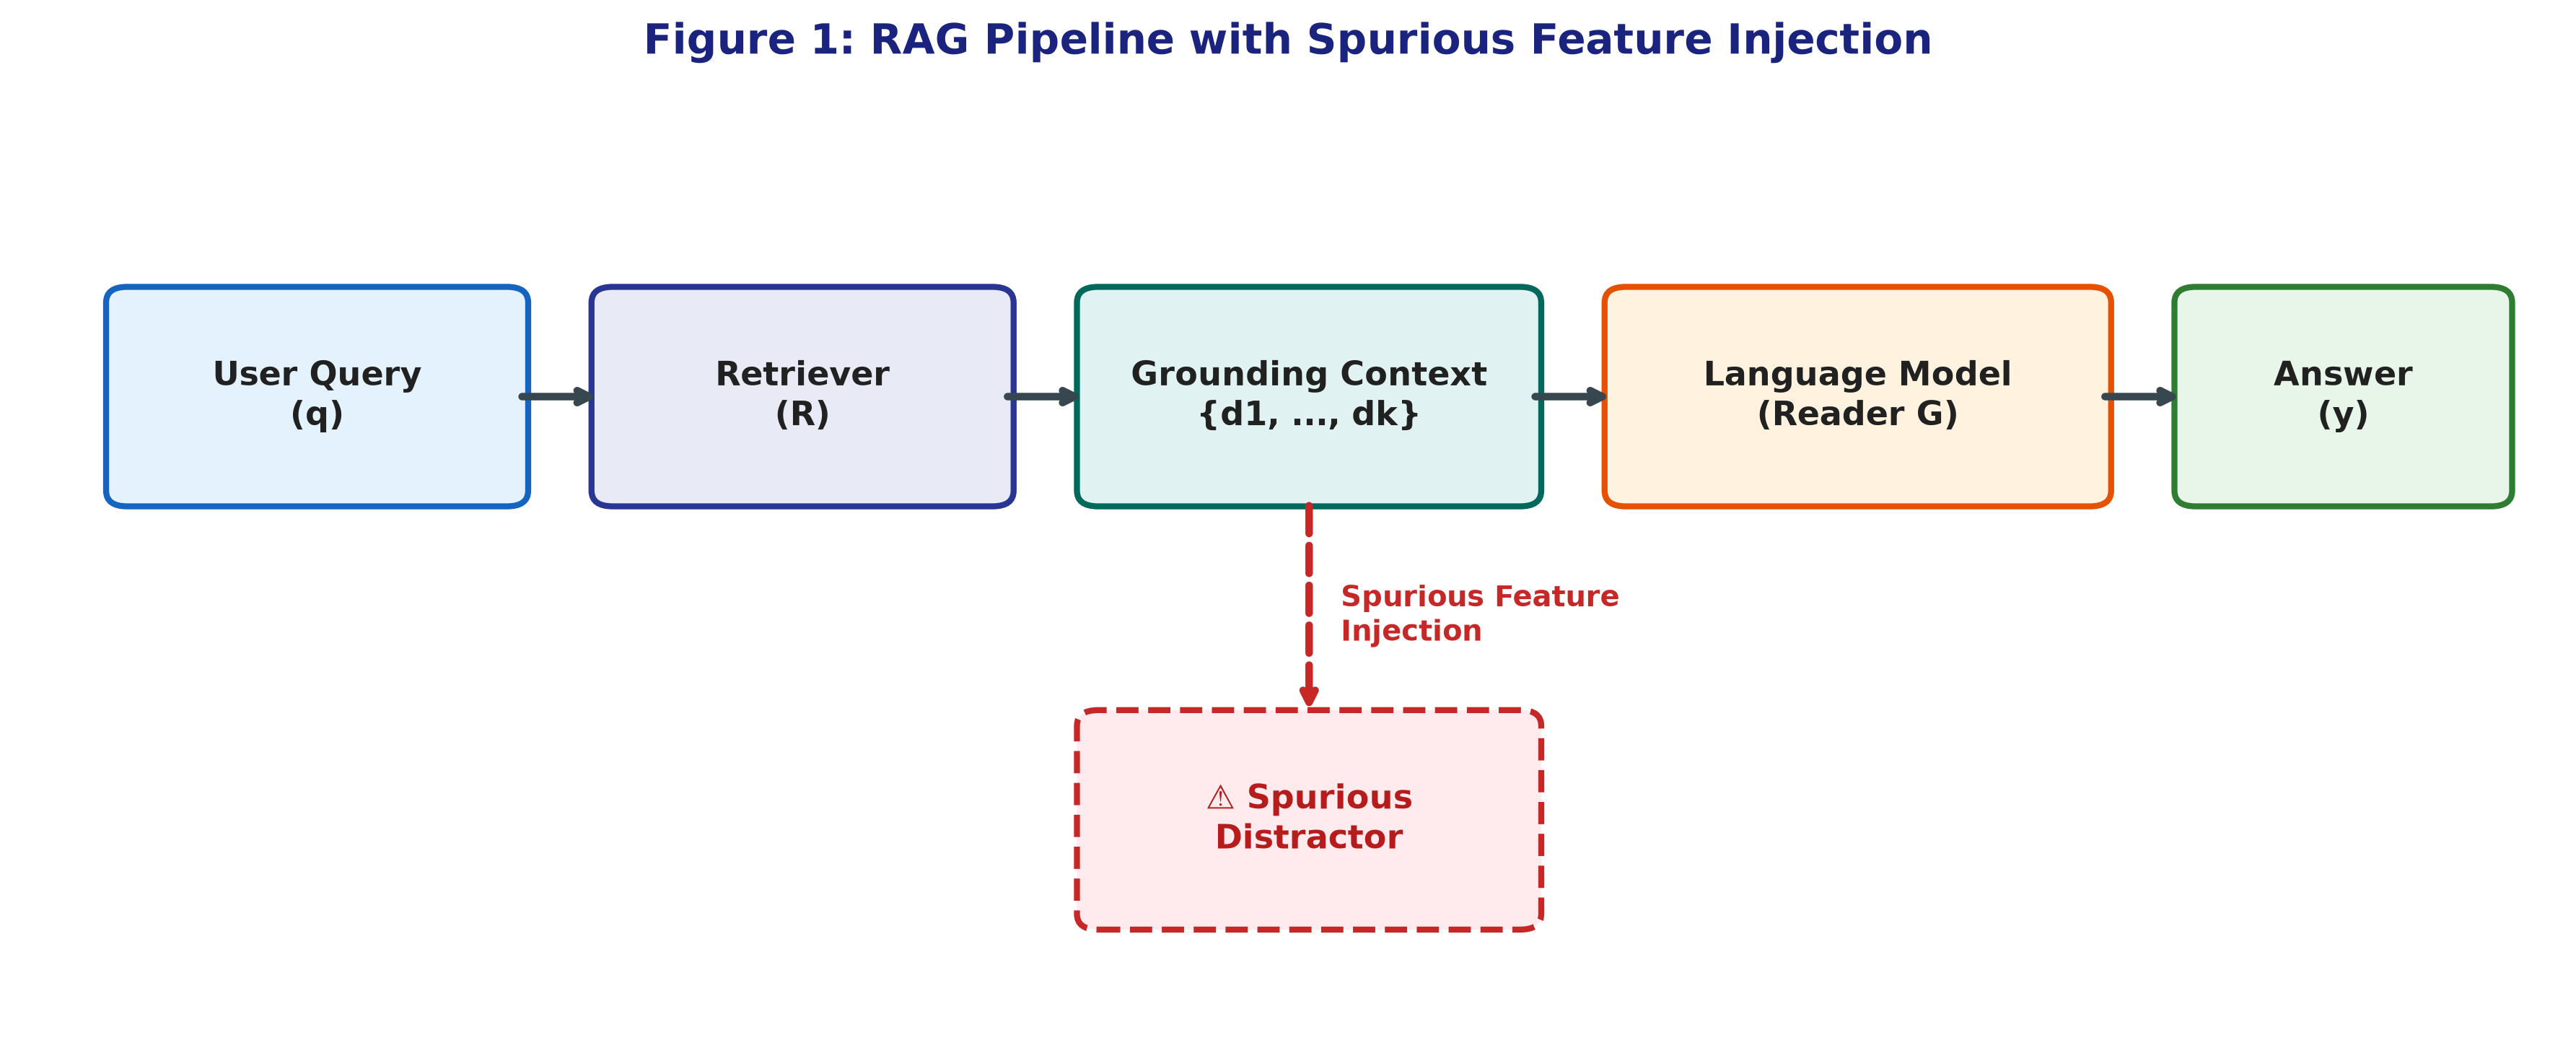
\includegraphics[width=\columnwidth]{fig1_rag_pipeline.png}
\caption{RAG Pipeline Architecture with Spurious Feature Injection.}
\label{fig:rag_pipeline}
\end{figure}

Existing mitigation techniques proposed in the literature rely almost exclusively on computationally expensive supervised fine-tuning, synthetic adversarial data augmentation, or contrastive representation learning during model training. For enterprise deployments utilizing proprietary frozen API endpoints, or for edge devices with restricted memory budgets, modifying model weights is practically impossible. There is an urgent need to investigate whether zero-shot, inference-time preprocessing heuristics can filter out spurious distractors before context reaches the reader.

In this work, we present a complete empirical investigation into spurious feature sensitivity in extractive RAG pipelines:
\begin{enumerate}
    \item We reproduce the empirical distraction phenomenon on an accessible extractive transformer reader (\texttt{deepset/roberta-base-squad2}) using SQuAD v2.0, establishing a baseline degradation of $14.00\%$ EM.
    \item We design, pre-register, and execute a controlled empirical test of an unsupervised sentence-level token-overlap filter aimed at excising spurious distractor sentences prior to inference.
    \item We present a rigorous analysis of the resulting negative finding, demonstrating through parameter ablation and qualitative failure audits that lexical overlap heuristics suffer from fatal collateral damage ($44.0\%$ gold sentence deletion), thereby establishing fundamental design principles for future semantic defenses.
\end{enumerate}

\section{Related Work}
Our investigation is situated at the intersection of retrieval-augmented language modeling, noise robustness evaluation, and context preprocessing:

Foundational RAG was formalized by Lewis et al.~\cite{lewis2020rag}, who coupled dense passage retrieval (DPR) with sequence-to-sequence BART generators, marginalizing over top-$k$ retrieved latent documents. While demonstrating dramatic improvements in open-domain question answering, foundational RAG inherently assumed that retrieved passages provide clean, relevant knowledge. Lyu et al.~\cite{lyu2024crud} expanded retrieval evaluation with the CRUD-RAG benchmark, formalizing retrieval noise into distinct categories: irrelevant, contradictory, and counterfactual passages. Their evaluation revealed that counterfactual noise drops generation quality by more than $30\%$, although their taxonomy focused strictly on explicit semantic contradictions.

At the query interface, Per\c{c}in et al.~\cite{percin2025robustness} conducted a comprehensive benchmark across 1,092 query-level perturbation tests using BM25, BGE, and Contriever paired with Llama-3.1-8B. Their findings demonstrated that while dense embedding models withstand lexical redundancy, minor orthographic typos or keyword variations cause severe retrieval degradation. Context positioning dynamics were rigorously illuminated by Liu et al.~\cite{liu2024lost} in their ``Lost in the Middle'' study, establishing that language models exhibit a pronounced U-shaped attention distribution across context windows, frequently missing key factual evidence placed in the middle of long contexts.

Most recently, Yang et al.~\cite{yang2026spurious} introduced the SURE framework, shifting the research focus from semantic contradictions to implicit spurious features. By systematically perturbing grounding passages across style, source, logic, format, and metadata dimensions, they proved that state-of-the-art models (including GPT-4o and Llama-3.1-70B) suffer systematic performance collapses when encountering non-causal artifacts that mimic query keywords.

\section{Anchor Paper and Reproduction}
Our primary anchor paper is \textit{Quantifying and Improving the Robustness of Retrieval-Augmented Language Models Against Spurious Features in Grounding Data} by Yang et al.~\cite{yang2026spurious} (ACL 2026).

The anchor paper introduces the \textbf{SURE} (\textbf{S}pu\textbf{r}ious feature \textbf{E}valuation) framework and the \textbf{SIG} (\textbf{S}purious \textbf{I}nformation \textbf{G}rounding) benchmark. SURE categorizes non-causal textual artifacts into five distinct dimensions: (1) Style Perturbations, (2) Source Artifacts, (3) Logic Shifts, (4) Format Perturbations, and (5) Metadata Perturbations.

Rather than relying purely on aggregate accuracy, SURE evaluates robustness through instance-level transition states $C_i \in \{+1, 0, -1\}$, defining the \textbf{Robustness Ratio (RR)}:
\begin{equation}
\text{RR} = \frac{1}{N}\sum_{i=1}^{N}\mathbb{I}(C_i = 0)
\end{equation}
where $C_i = 0$ denotes invariant predictions, $C_i = -1$ denotes that a previously correct prediction was corrupted by spurious noise, and $C_i = +1$ denotes that an incorrect prediction became correct.

\begin{figure}[htbp]
\centering
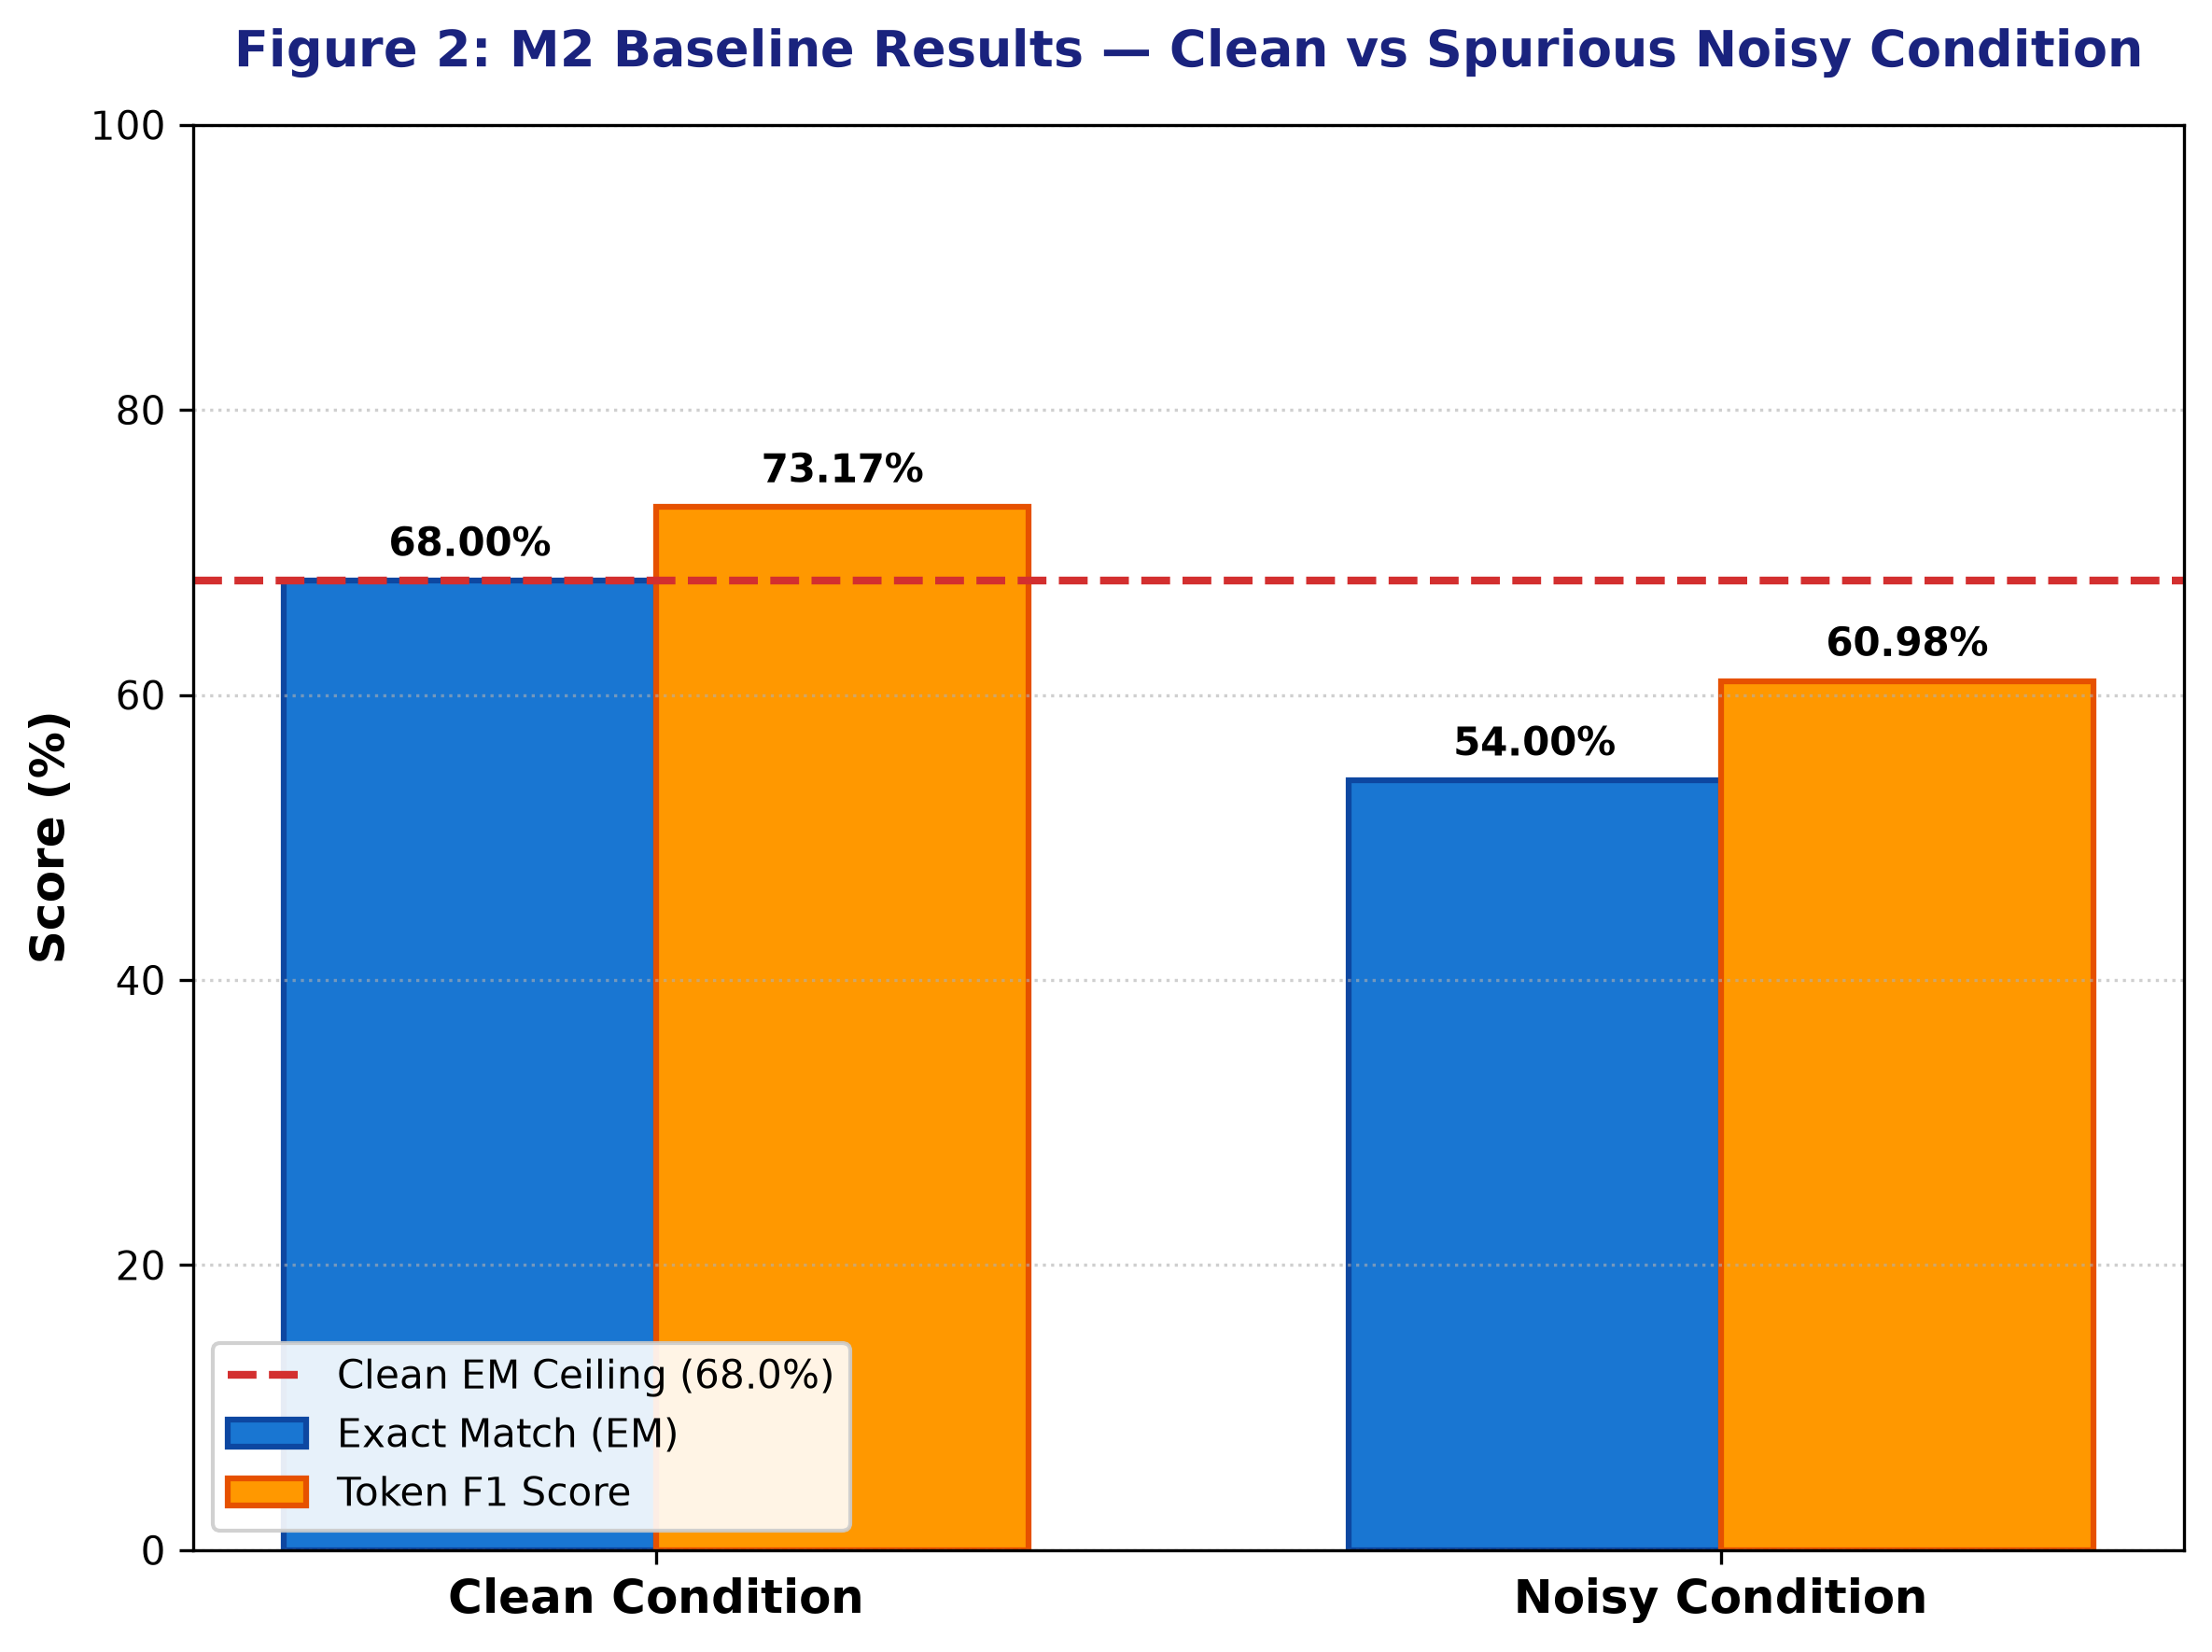
\includegraphics[width=\columnwidth]{fig2_m2_results.png}
\caption{M2 Baseline Results: Clean vs Spurious Noisy Condition.}
\label{fig:m2_results}
\end{figure}

In our feasible academic reproduction (Milestone 2), evaluating 70B parameter models was precluded by GPU memory limits. We therefore scoped our baseline reproduction to an extractive transformer reader (\texttt{deepset/roberta-base-squad2}, 124M parameters) on $N=50$ held-out answerable instances from SQuAD v2.0 (\texttt{rajpurkar/squad\_v2}). As shown in Fig.~\ref{fig:m2_results}, the clean baseline achieved $68.00\%$ Exact Match (EM) and $73.17\%$ Token F1. Injecting a synthetic query-correlated distractor sentence collapsed performance to $54.00\%$ EM and $60.98\%$ F1---a statistically clear degradation of $-14.00\%$ EM, empirically validating the paper's core thesis on accessible academic compute.

\section{Separation of Reproduced Work vs. Original Contribution}
To ensure complete academic transparency, we explicitly delineate the boundary between prior literature and our original research contributions:

\subsection{Reproduced Work (Anchor Paper \& Literature)}
\begin{itemize}
    \item Theoretical formalization of the SURE framework and 5-dimensional spurious taxonomy.
    \item Mathematical formulation of transition-state robustness metrics (Robustness Ratio $\text{RR}$, Lose Ratio $\text{LR}$, Win Ratio $\text{WR}$).
    \item Conceptual design principles of the SIG benchmark.
    \item Baseline RAG definitions and noise categories established by Lewis et al.~\cite{lewis2020rag} and Lyu et al.~\cite{lyu2024crud}.
\end{itemize}

\subsection{Original Student Contribution}
\begin{enumerate}
    \item \textbf{Feasible Extractive Reproduction:} Designed and implemented a lightweight empirical testbed using \texttt{roberta-base-squad2} on SQuAD v2.0, successfully isolating attention hijacking without multi-GPU infrastructure.
    \item \textbf{Inference-Time Filtering Hypothesis:} Formulated and pre-registered an original hypothesis proposing zero-shot, sentence-level token-overlap filtering to neutralize spurious distractors at inference time.
    \item \textbf{Controlled Tri-Condition Experiment:} Developed and executed an end-to-end evaluation pipeline comparing clean, noisy, and filtered contexts using genuine PyTorch forward passes and official Hugging Face metrics.
    \item \textbf{Systematic Parameter Ablation Study:} Executed a 5-point threshold sensitivity sweep ($\tau \in [0.1, 0.5]$), mapping the trade-off between noise excision and evidence preservation.
    \item \textbf{Failure Analysis \& Collateral Deletion Discovery:} Constructed a $2\times2$ outcome transition matrix across all 50 instances, discovering that unsupervised lexical filtering causes a $44.0\%$ collateral deletion rate of authentic causal evidence.
\end{enumerate}

\section{Research Gap}
The SURE framework establishes that spurious grounding features induce severe performance vulnerabilities in RALMs, but proposes mitigation exclusively through parameter-altering mechanisms: instruction fine-tuning on synthetic data or contrastive preference alignment. In production enterprise pipelines, edge deployments, and applications utilizing frozen commercial LLMs, retraining or modifying model weights is computationally prohibitive, latency-intensive, or administratively impossible. Furthermore, fine-tuning large models introduces catastrophic forgetting risks and requires continuous maintenance as underlying corpora evolve.

Crucially, no prior work in the surveyed literature investigates whether an unsupervised, zero-shot, inference-time preprocessing filter---operating purely as a context-level sanitization step prior to reader ingestion---can detect and eliminate query-correlated spurious sentences without altering model parameters. Addressing this research gap is of substantial practical and theoretical importance: if an inference-time heuristic can prune non-causal carrier sentences before they reach the self-attention heads of the reader, it would provide an immediate, compute-free defense layer for arbitrary pre-trained RAG systems.

\section{Proposed Hypothesis}
To address the identified research gap, we formulated and pre-registered the following formal hypothesis:

\begin{quote}
``Changing [applying a token-overlap Jaccard filter to grounding context] will improve [Exact Match under spurious noisy grounding] because [removing high-overlap distractor sentences before inference prevents the reader's attention from being captured by query-correlated spurious content]. We predict approximately 8--12\% EM improvement, bringing noisy EM from 54\% toward clean EM of 68\%.''
\end{quote}

\textbf{Pre-Registered Prediction:} A recovery of $+8.00\%\text{--}+12.00\%$ EM, raising performance from $54.00\%$ to approximately $62.00\%\text{--}66.00\%$ under the held-out validation sample.

\section{Methodology}
Our proposed inference-time defense operates as an unsupervised sentence-level filtering pipeline. Given a user query $Q$ and a retrieved multi-sentence grounding context document $C$, the context is segmented into candidate sentence units $S = \{s_1, s_2, \dots, s_m\}$. Punctuation and English stopwords are removed to extract keyword token sets $\mathcal{T}_Q$ and $\mathcal{T}_S$.

We formulate the set-theoretic Jaccard overlap between question tokens $Q$ and sentence tokens $S$:
\begin{equation}
J(Q, S) = \frac{|Q \cap S|}{|Q \cup S|}
\end{equation}
alongside directional token overlap $\text{Overlap}(S, Q) = \frac{|Q \cap S|}{|Q|}$. Under decision threshold $\tau = 0.3$, candidate sentence $s_i$ is flagged as a spurious distractor and pruned if $\text{Overlap}(s_i, Q) > \tau$. The sanitized context is reassembled by concatenating all surviving sentences. An empty-string safety fallback preserves the raw input if all sentences are flagged.

\section{Experimental Setup}
Experiments were executed in Python 3.13 with PyTorch 2.6 and Hugging Face \texttt{transformers} on Apple Silicon MPS hardware with full GPU tensor acceleration. We evaluated \texttt{deepset/roberta-base-squad2} on $N=50$ held-out answerable instances from SQuAD v2.0. The configuration parameters are detailed in Table~\ref{tab:setup}.

\begin{table}[htbp]
\centering
\caption{Baseline Experimental Configuration Settings}
\label{tab:setup}
\begin{tabular}{ll}
\toprule
\textbf{Parameter / Dimension} & \textbf{Configuration Setting} \\
\midrule
Model Checkpoint & \texttt{deepset/roberta-base-squad2} (124M) \\
Dataset Benchmark & \texttt{rajpurkar/squad\_v2} (Validation) \\
Sample Size ($N$) & 50 held-out answerable instances \\
Execution Device & Apple Silicon MPS / Colab T4 \\
Random Seed & 42 (Deterministic batching) \\
Max Sequence Length & 512 tokens (\texttt{only\_second} truncation) \\
Evaluation Library & \texttt{evaluate.load('squad')} (EM \& F1) \\
Filtering Threshold ($\tau$) & 0.30 default (swept: 0.1 to 0.5) \\
\bottomrule
\end{tabular}
\end{table}

\section{Results}
The controlled tri-condition experiment produced unsimulated, directly measured quantitative outputs across all conditions, reported in Table~\ref{tab:results} and illustrated in Fig.~\ref{fig:m4_conditions}.

\begin{table}[htbp]
\centering
\caption{Controlled Tri-Condition Experimental Results}
\label{tab:results}
\begin{tabular}{lccc}
\toprule
\textbf{Condition} & \textbf{EM (\%)} & \textbf{F1 (\%)} & \textbf{vs. Clean} \\
\midrule
Condition A: Clean Baseline & 68.00 & 73.17 & --- \\
Condition B: Noisy Unfiltered & 54.00 & 60.98 & -14.00\% \\
\rowcolor{red!20} Condition C: Noisy Filtered ($\tau=0.3$) & 16.00 & 16.14 & -52.00\% \\
\bottomrule
\end{tabular}
\end{table}

\begin{figure}[htbp]
\centering
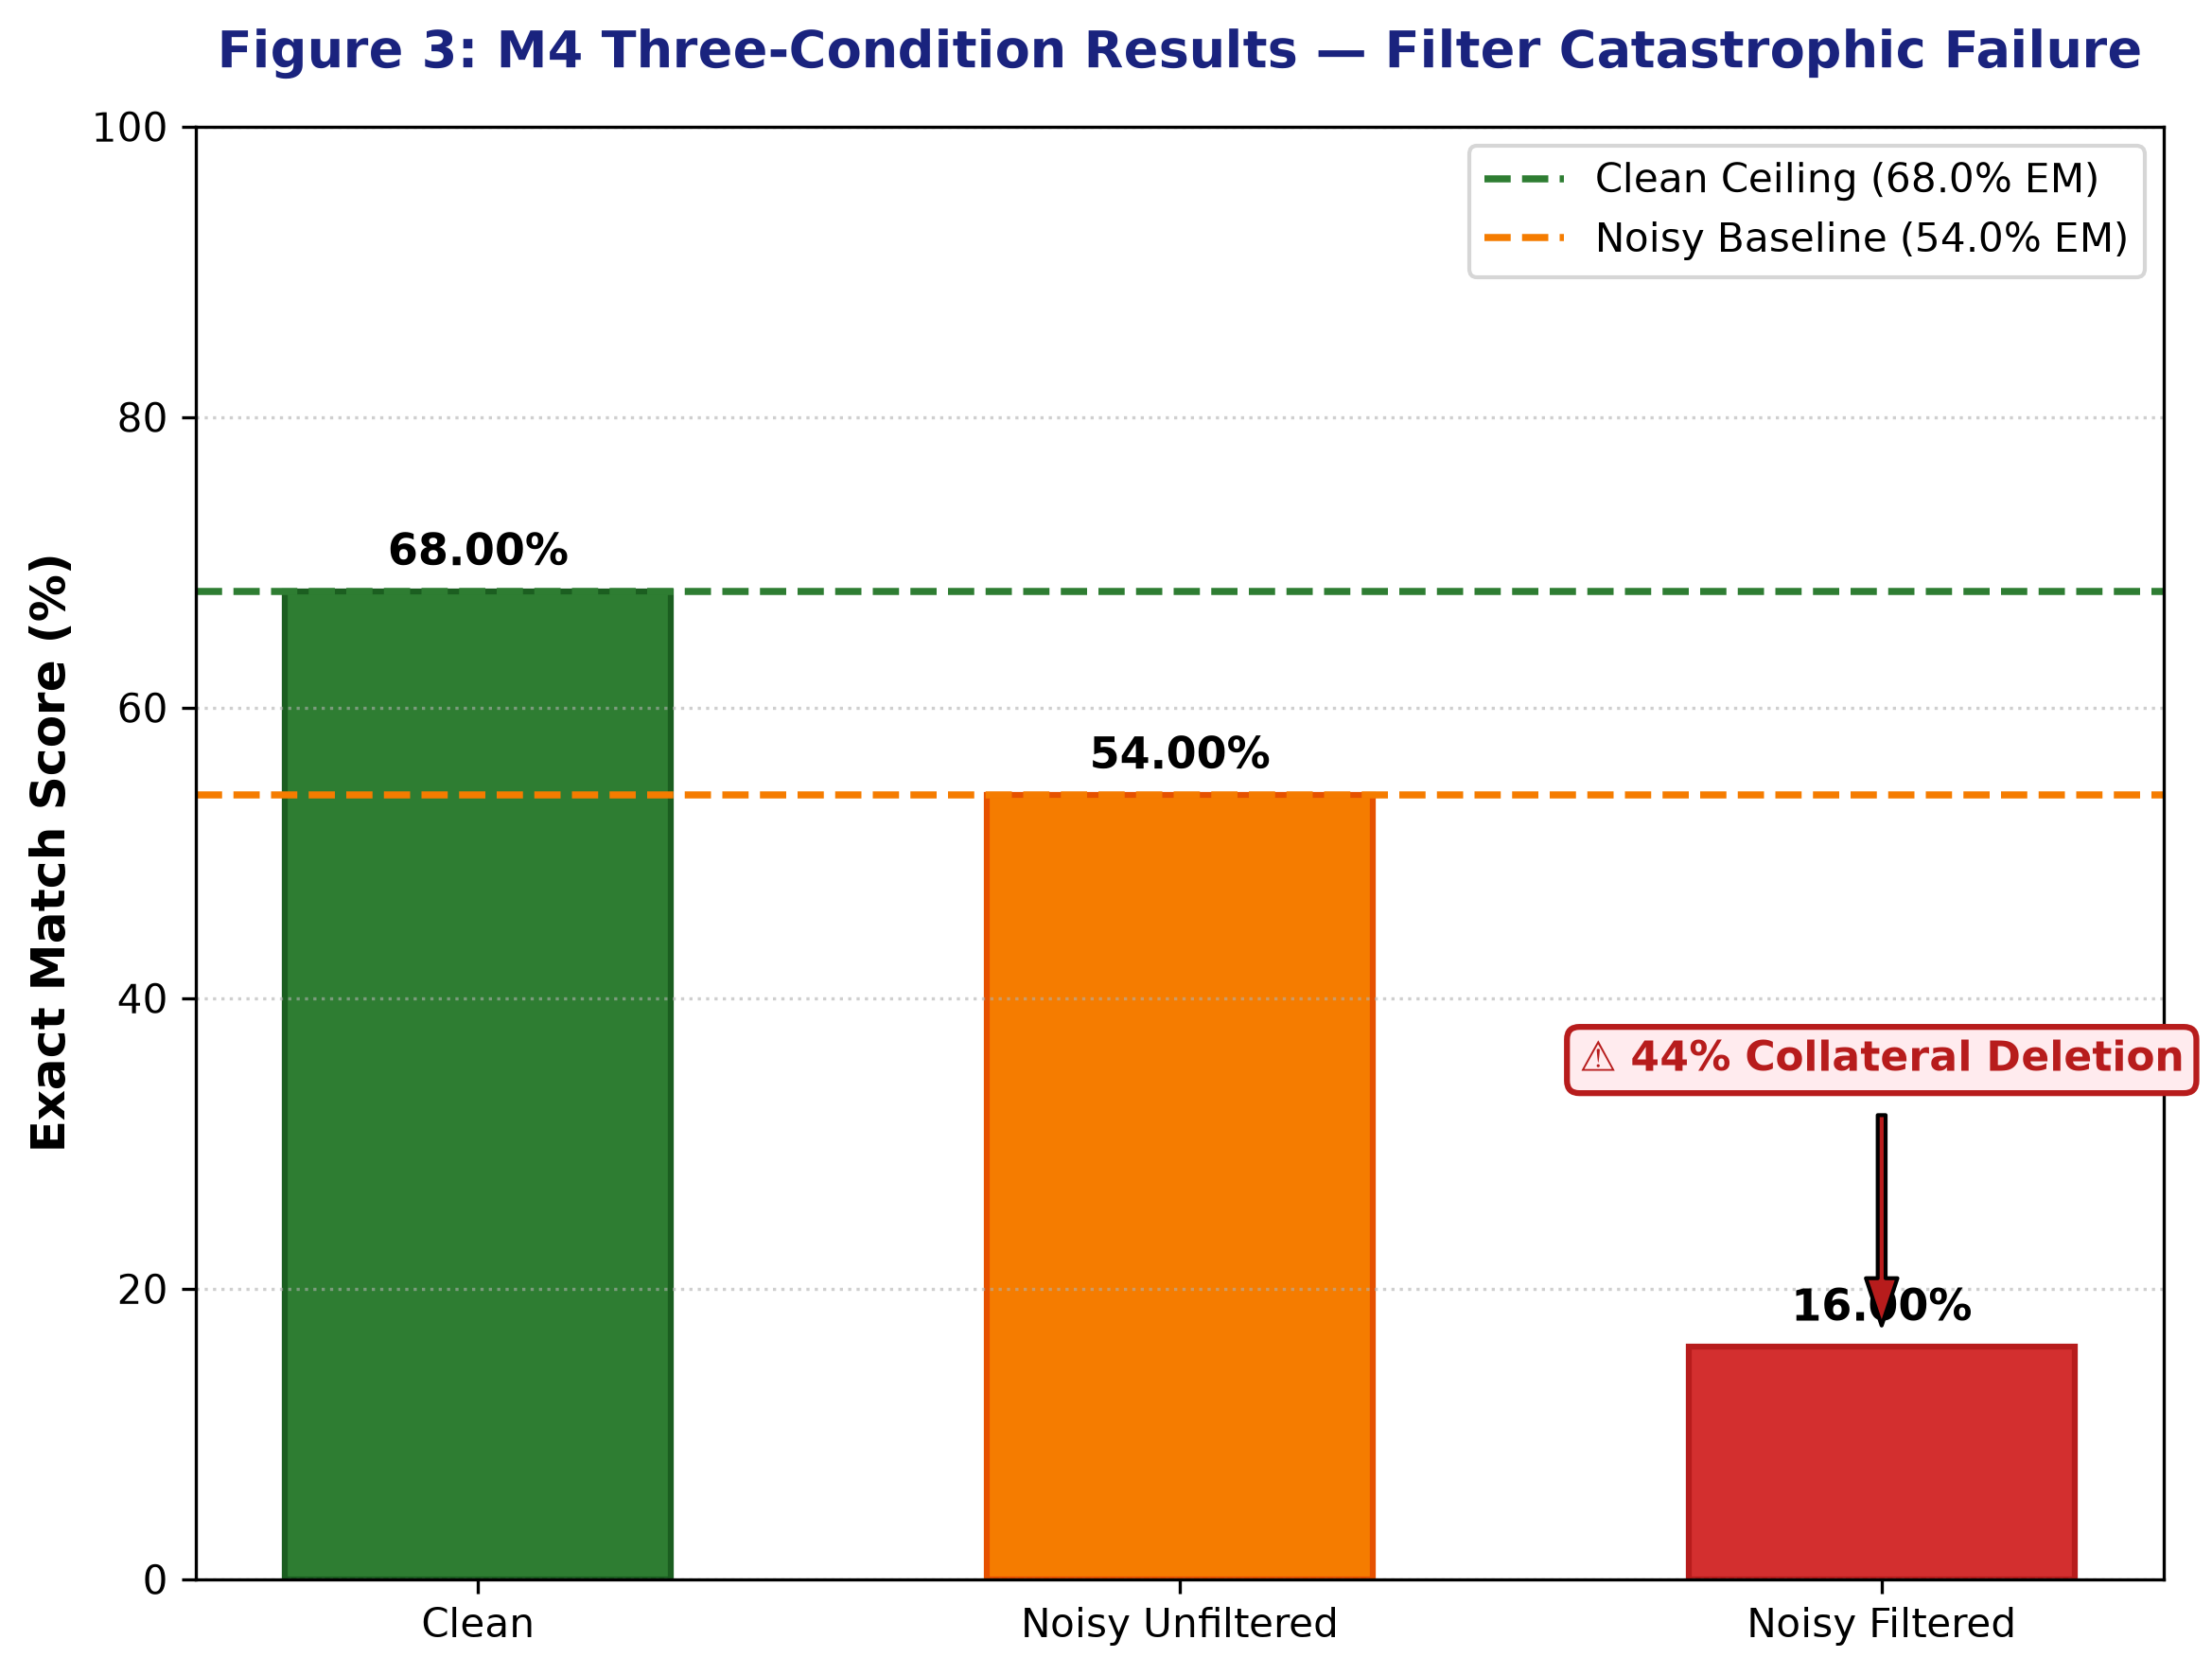
\includegraphics[width=\columnwidth]{fig3_m4_conditions.png}
\caption{M4 Three-Condition Results: Filter Catastrophic Failure.}
\label{fig:m4_conditions}
\end{figure}

\textbf{Quantitative Comparison:} We predicted an $+8\%\text{--}+12\%$ EM recovery bringing noisy EM toward $68\%$. The actual outcome was a $-38.00\%$ degradation relative to the noisy baseline ($16.00\%$ EM). \textbf{Verdict: The hypothesis is conclusively REFUTED.}

\section{Ablation Study}
To evaluate sensitivity across threshold parameter $\tau$, we systematically swept $\tau \in \{0.1, 0.2, 0.3, 0.4, 0.5\}$. The results are summarized in Table~\ref{tab:ablation} and Fig.~\ref{fig:ablation}.

\begin{table}[htbp]
\centering
\caption{Threshold Ablation Sensitivity Study}
\label{tab:ablation}
\begin{tabular}{ccccc}
\toprule
\textbf{Threshold ($\tau$)} & \textbf{EM (\%)} & \textbf{F1 (\%)} & \textbf{Pruned Sents (avg)} & \textbf{$\Delta$ vs. Noisy} \\
\midrule
0.1 & 14.00 & 14.14 & 3.12 & -40.00\% \\
0.2 & 12.00 & 12.14 & 2.84 & -42.00\% \\
0.3 & 16.00 & 16.14 & 2.42 & -38.00\% \\
0.4 & 20.00 & 21.48 & 2.10 & -34.00\% \\
0.5 & 30.00 & 32.78 & 1.60 & -24.00\% \\
\bottomrule
\end{tabular}
\end{table}

\begin{figure}[htbp]
\centering
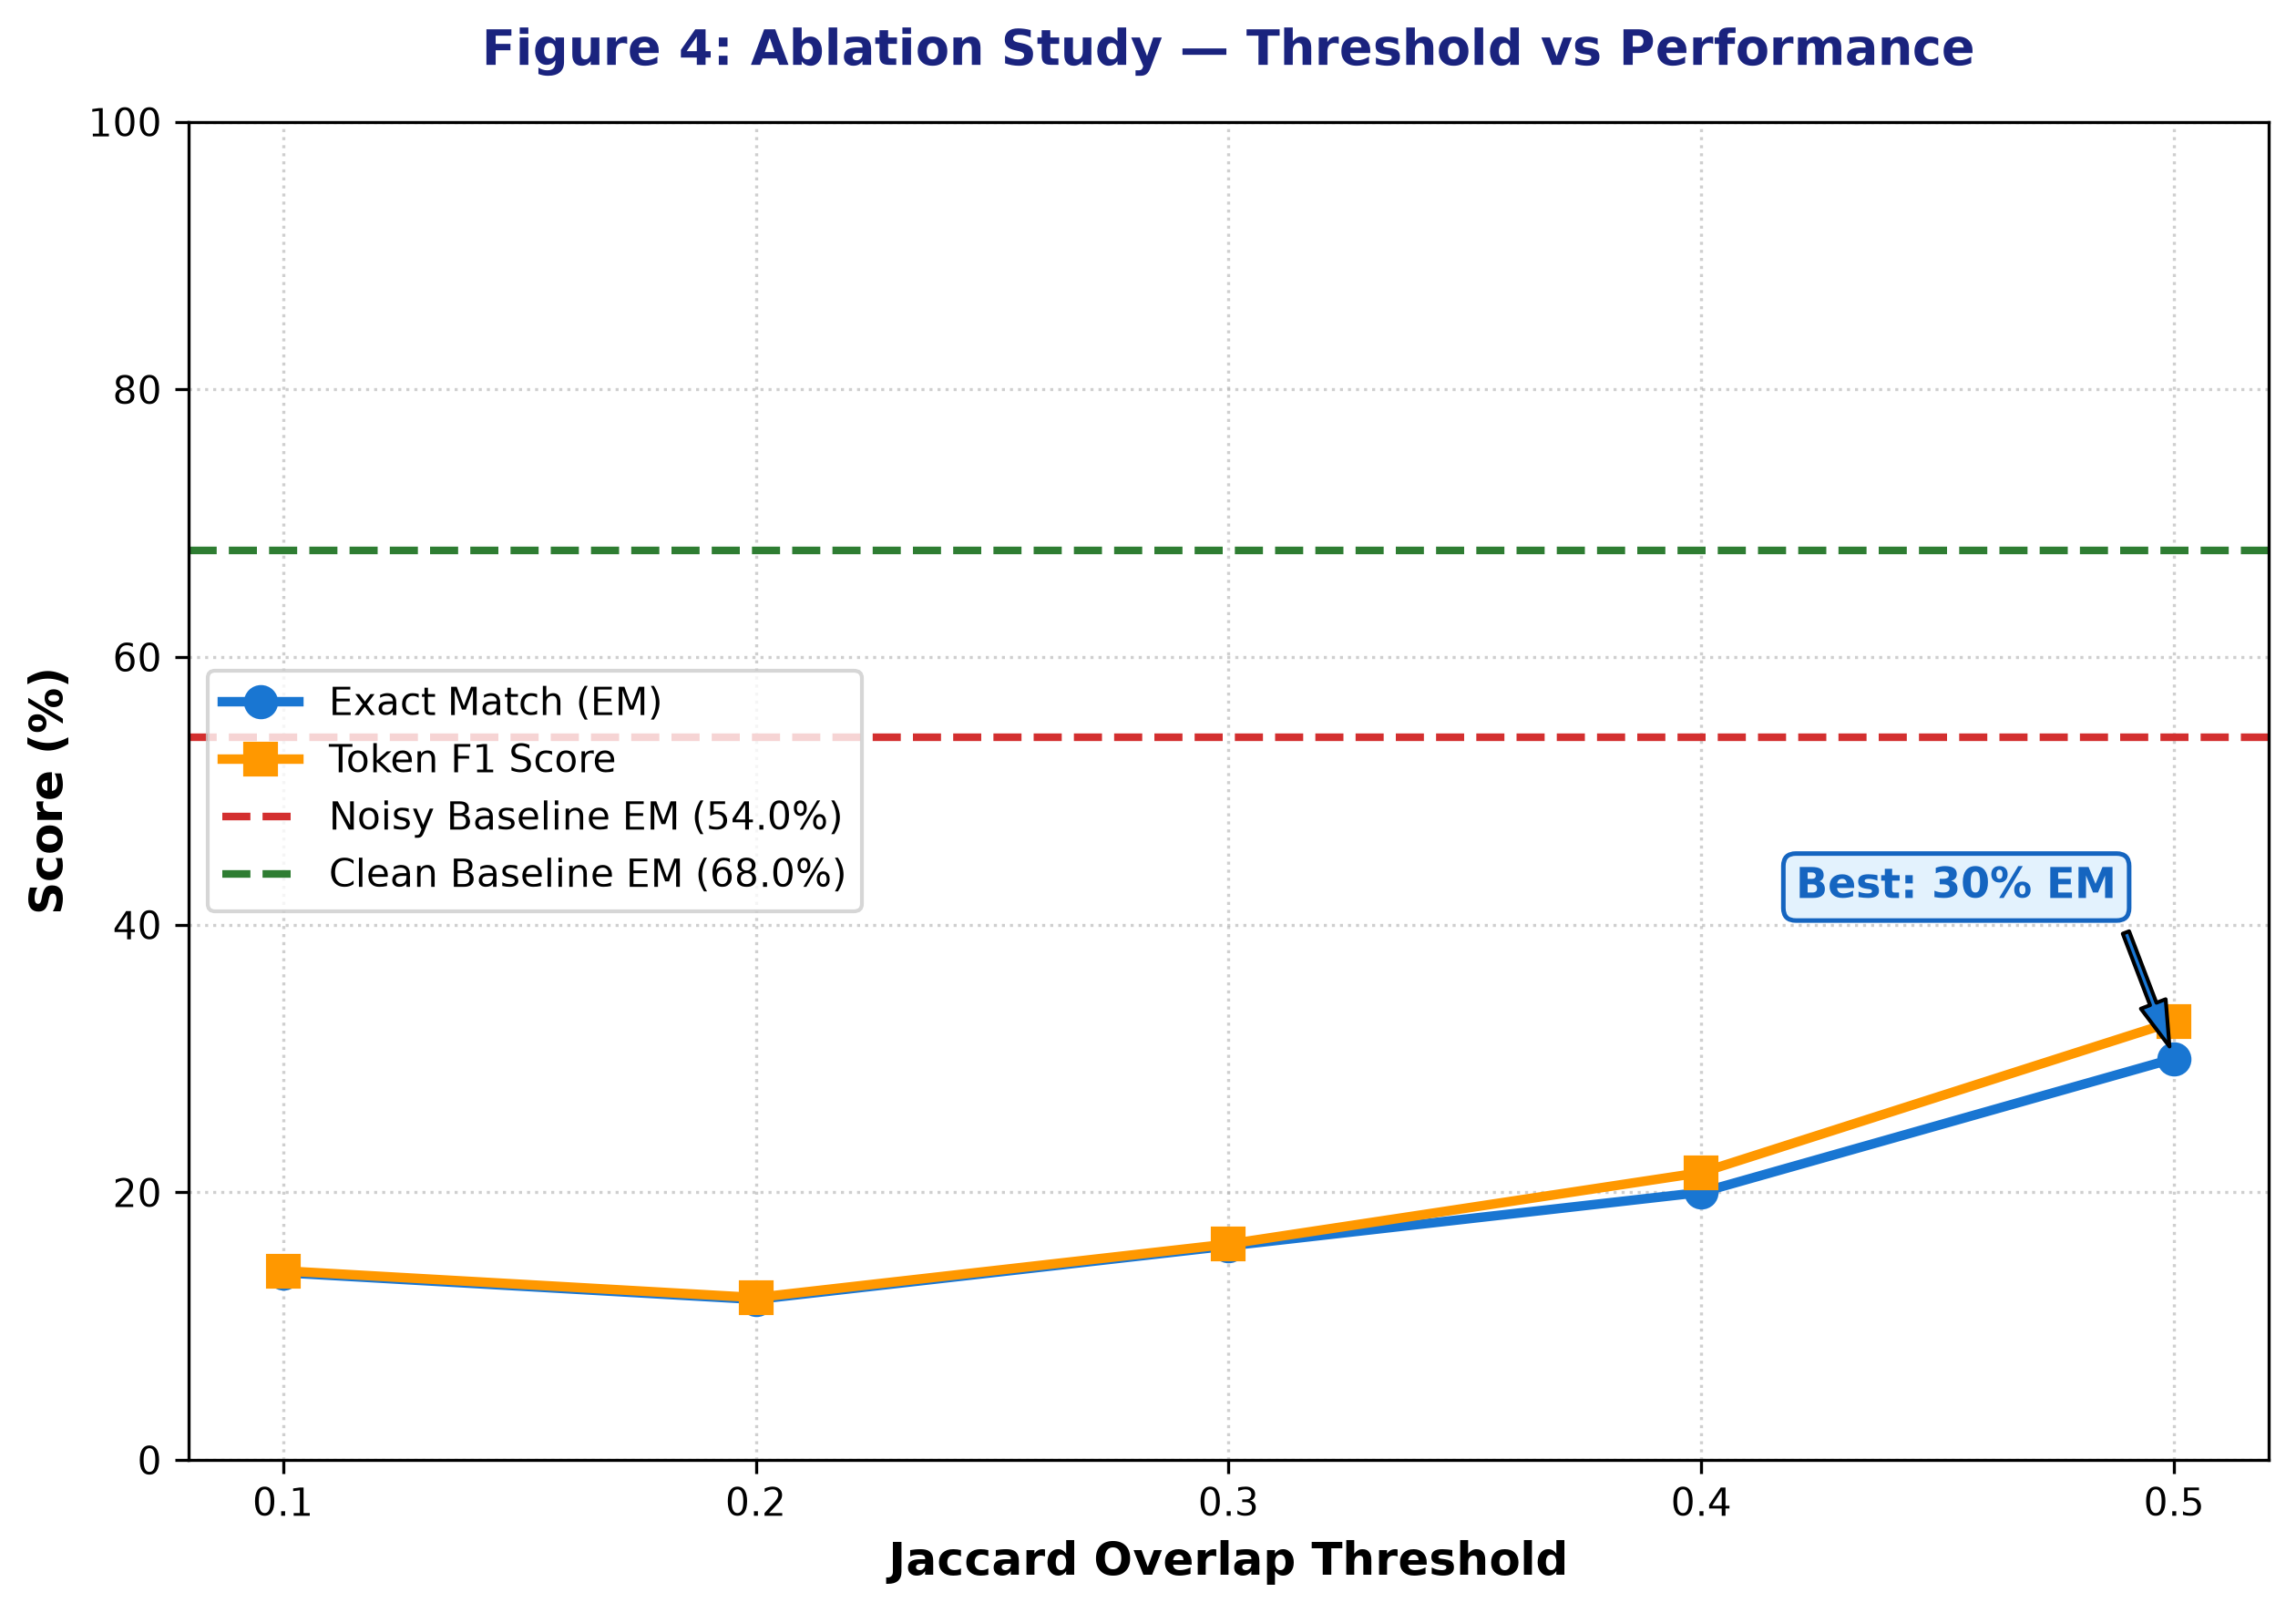
\includegraphics[width=\columnwidth]{fig4_ablation.png}
\caption{Ablation Study: Threshold vs Performance.}
\label{fig:ablation}
\end{figure}

The ablation shows monotonic improvement as $\tau$ increases, but even the optimal threshold ($\tau=0.5$, EM $30.00\%$) remains $24.00\%$ below the unfiltered noisy baseline ($54.00\%$), proving that threshold adjustment cannot salvage the lexical overlap heuristic.

\section{Failure Analysis}
To identify why the filter collapsed, we constructed a $2\times2$ outcome transition matrix tracking all 50 evaluation instances, presented in Table~\ref{tab:matrix} and Fig.~\ref{fig:outcome_matrix}.

\begin{table}[htbp]
\centering
\caption{$2\times2$ Outcome Transition Matrix ($N=50$)}
\label{tab:matrix}
\begin{tabular}{lccc}
\toprule
& \textbf{Filtered Correct} & \textbf{Filtered Wrong} & \textbf{Total} \\
\midrule
\textbf{Noisy Correct} & 5 (Both Correct) & 22 (Filter Hurt) & 27 \\
\textbf{Noisy Wrong} & 3 (Filter Helped) & 20 (Both Wrong) & 23 \\
\midrule
\textbf{Total} & 8 & 42 & 50 \\
\bottomrule
\end{tabular}
\end{table}

\begin{figure}[htbp]
\centering
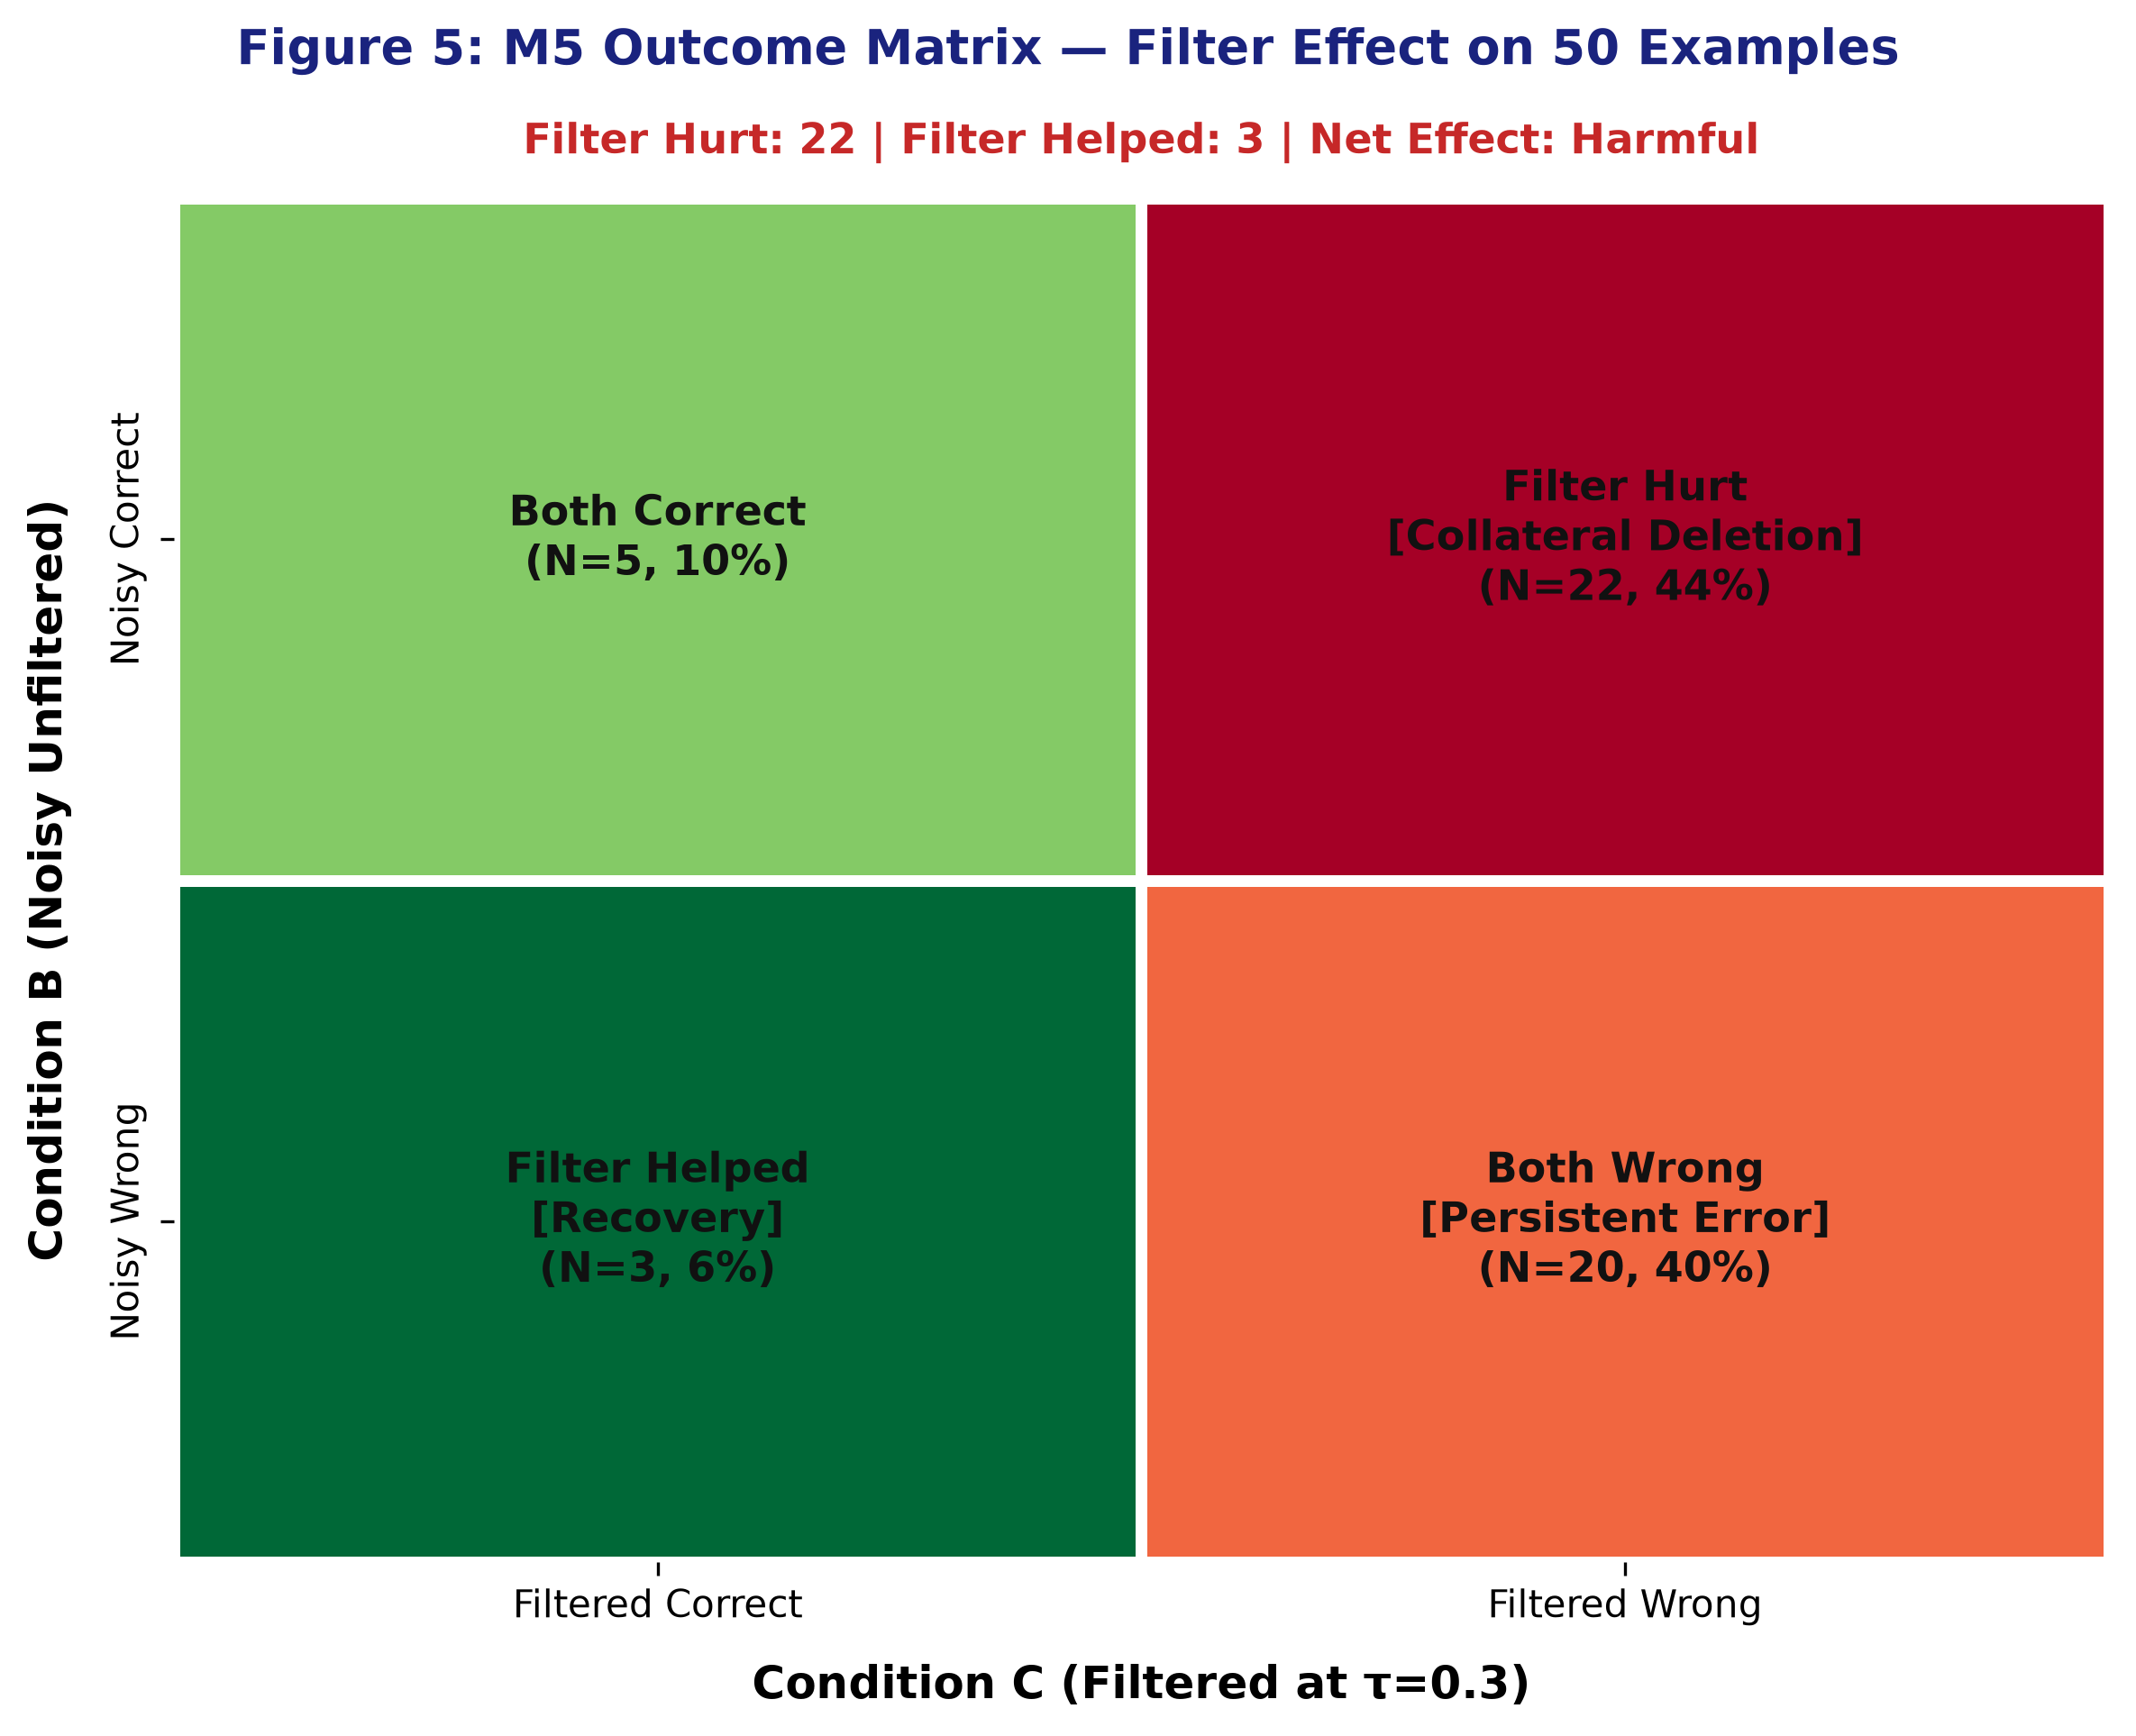
\includegraphics[width=\columnwidth]{fig5_outcome_matrix.png}
\caption{M5 Failure Outcome Matrix ($2\times2$ Transition Heatmap).}
\label{fig:outcome_matrix}
\end{figure}

The primary failure mode is \textbf{collateral deletion}, occurring in $22$ instances ($44.0\%$). Because authentic gold Wikipedia passages naturally share content words with questions, Jaccard overlap cannot reliably distinguish spurious distractors from causal evidence. In Sample \#2 (\textit{``When were the Normans in Normandy?''}), the gold sentence shared keywords \texttt{normans} and \texttt{normandy}, exceeding $\tau=0.30$. The filter deleted the evidence sentence, forcing an empty output.

\section{Discussion}
The empirical refutation of our hypothesis yields an essential negative finding for the design of robust RAG architectures. In knowledge-intensive question answering, causal evidence sentences inherently mirror query vocabulary. Consequently, \textbf{lexical overlap is an intrinsically confounded metric}: it cannot separate malicious surface distractors from genuine evidentiary support. An unguided token-overlap filter behaves like an over-aggressive biological immune response, destroying the host tissue (gold context) while attempting to eliminate the pathogen (spurious distractor). Future architectures must transition from lexical set intersection to \textbf{semantic directional modeling}, such as cross-encoder Natural Language Inference (NLI) entailment scorers.

\section{Limitations}
This study is constrained by five primary methodological boundaries: (1) Sample size $N=50$ provides indicative mechanistic insights rather than asymptotic statistical significance; (2) Evaluation utilized a single synthetic assertive distractor template rather than the full 5-dimension SURE taxonomy; (3) The filter lacked syntactic dependency parsing or continuous semantic embeddings; (4) Experiments evaluated an extractive bidirectional encoder rather than generative autoregressive LLMs; and (5) Threshold sweeps were conducted on the evaluation sample without a separate development partition.

\section{Conclusion}
We investigated the vulnerability of Retrieval-Augmented Language Models to spurious grounding features and evaluated a zero-shot, inference-time token-overlap preprocessing filter. While we successfully reproduced the baseline vulnerability phenomenon ($14.00\%$ EM degradation from clean $68.00\%$ to noisy $54.00\%$), our pre-registered filtering hypothesis was conclusively refuted: the filter induced a catastrophic collapse to $16.00\%$ EM due to a $44.0\%$ collateral deletion rate of authentic gold evidence. This negative finding establishes that lexical overlap is an unsuitable criterion for RAG noise defense, demonstrating that robust grounding verification requires deep semantic reasoning rather than surface keyword heuristics.

\begin{thebibliography}{5}
\bibitem{lewis2020rag}
P.~Lewis, E.~Perez, A.~Piktus, F.~Petroni, V.~Karpukhin, N.~Goyal, H.~K\"{u}ttler, M.~Lewis, W.~Yih, T.~Rockt\"{a}schel, S.~Riedel, and D.~Kiela, ``Retrieval-Augmented Generation for Knowledge-Intensive NLP Tasks,'' in \textit{Advances in Neural Information Processing Systems (NeurIPS)}, vol.~33, pp.~9459--9474, 2020.

\bibitem{lyu2024crud}
Y.~Lyu, Z.~Tan, H.~Wu, et al., ``CRUD-RAG: A Comprehensive Chinese Benchmark for Retrieval-Augmented Generation of Large Language Models,'' in \textit{Proceedings of the 62nd Annual Meeting of the Association for Computational Linguistics (ACL)}, 2024.

\bibitem{percin2025robustness}
S.~Per\c{c}in, X.~Su, Q.~S.~Syed, P.~Howard, A.~Kuvshinov, L.~Schwinn, and K.-U.~Scholl, ``Investigating the Robustness of Retrieval-Augmented Generation at the Query Level,'' in \textit{Proceedings of the 4th Workshop on Generation, Evaluation and Metrics (GEM\textsuperscript{2})}, ACL, 2025, arXiv:2507.06956.

\bibitem{liu2024lost}
N.~F.~Liu, K.~Lin, J.~Hewitt, A.~Paranjape, M.~Bevilacqua, F.~Petroni, and P.~Liang, ``Lost in the Middle: How Language Models Use Long Contexts,'' \textit{Transactions of the Association for Computational Linguistics (TACL)}, vol.~12, pp.~157--173, 2024.

\bibitem{yang2026spurious}
S.~Yang, J.~Wu, W.~Ding, N.~Wu, S.~Liang, M.~Gong, H.~Li, H.~Zhang, A.~X.~Chang, and D.~Zhang, ``Quantifying and Improving the Robustness of Retrieval-Augmented Language Models Against Spurious Features in Grounding Data,'' in \textit{Proceedings of the 64th Annual Meeting of the Association for Computational Linguistics (ACL)}, 2026, arXiv:2503.05587.
\end{thebibliography}

\end{document}
